\begin{code}[hide]
module vqupit.sections.two-routes where

open import Data.Nat using (ℕ)
open import Notations using (₁₊ ; ₂₊)
open import Word.Base using (Word ; WRel ; ε ; _•_ ; _^_)

infixl 9 _↑ _↓
infix 4 _SRel,_===_ _≈_
infix 1 begin_
infixr 2 _≈⟨_⟩_
infix 3 _∎
infixl 3 cleft_ cright_

private variable
  n : ℕ

postulate
  Gen : ℕ → Set
  H S CZ : ∀ {n} → Word (Gen n)
  _↑ _↓ : ∀ {n} → Word (Gen n) → Word (Gen n)
  _≈_ : ∀ {n} → Word (Gen n) → Word (Gen n) → Set
  begin_ : ∀ {n} {w v : Word (Gen n)} → w ≈ v → w ≈ v
  _≈⟨_⟩_ : ∀ {n} (w : Word (Gen n)) {v u} → w ≈ v → v ≈ u → w ≈ u
  _∎ : ∀ {n} (w : Word (Gen n)) → w ≈ w
  sym assoc right-unit cleft_ cright_ axiom : ∀ {ℓ} {A : Set ℓ} → A
\end{code}
\section{Qupit Circuits and the Verification Strategy}\label{sec:two-routes}

We first specify the intended circuit language, then distinguish the
semantic layers that the verification treats separately.  Throughout,
\emph{the original rules} means Figure~1 of the qupit
presentation~\cite{bian2026qudit}; figures in this paper have their own
numbering.

\subsection{Qupit Clifford operators}\label{sec:operators}

Fix an odd prime $p$ and let $\omega = e^{2\pi i/p}$.  A \emph{qupit} is
a $p$-dimensional quantum system with computational basis
$\ket{0},\dots,\ket{p-1}$, indices read in $\Zp$.  The single-qupit Pauli
operators are $X\ket{j} = \ket{j+1}$ and $Z\ket{j} = \omega^{j}\ket{j}$;
the $n$-qupit Pauli group $\Pauli$ is generated by tensor products of $X$
and $Z$ together with the phases $\omega^t$.  The $n$-qupit Clifford
group $\Cliff$ is generated, under composition and tensor product, by the
gates of Table~\ref{tab:gates}, whose qubit counterparts are shown for
comparison, together with the phases $\omega^t$.  We follow the qupit paper's conventions
\cite{bian2026qudit}: the $\tfrac12$ in $S$ is the inverse of $2$ in
$\Zp$, and $H$ carries the global phase $\delta_p = i^{-(p-1)/2}$, which
fixes the Fourier gate's scalar convention.  This table specifies
the intended matrices; the formal semantics below uses finite-field
algebra instead.

\begin{table}[h]
\caption{The Clifford generators for qubits and for qupits (odd prime $p$).}
\label{tab:gates}
\centering
\begin{tabular}{lll}
\toprule
 & qubit ($p = 2$) & qupit (odd prime $p$) \\
\midrule
$H$  & $\frac{1}{\sqrt2}\begin{pmatrix}1&1\\1&-1\end{pmatrix}$
     & $\ket{j} \mapsto \tfrac{\delta_p}{\sqrt p}\sum_k \omega^{jk}\ket{k}$ \\[2ex]
$S$  & $\begin{pmatrix}1&0\\0&i\end{pmatrix}$
     & $\ket{j} \mapsto \omega^{j(j-1)/2}\,\ket{j}$ \\[2ex]
$CZ$ & $\mathrm{diag}(1,1,1,-1)$
     & $\ket{j}\ket{l} \mapsto \omega^{jl}\,\ket{j}\ket{l}$ \\
\bottomrule
\end{tabular}
\end{table}

Three quotients of $\Cliff$ matter.  Writing $\langle\omega\rangle$ for
the scalars, $\PCliff = \Cliff/\langle\omega\rangle$ is the
\emph{projective} Clifford group and $\PPauli =
\Pauli/\langle\omega\rangle \cong \Zp^{2n}$ the projective Pauli group,
an abelian group in which $X$ and $Z$ commute.  Conjugation by a Clifford
operator permutes Paulis and preserves their commutation phases, so
modulo Paulis a Clifford operator is a symplectic matrix: $\Cliff/\Pauli
\cong \PCliff/\PPauli \cong \Sp$, the symplectic group of the
$2n$-dimensional $\Zp$-vector space $\Zp^{2n}$ with its standard
symplectic form~\cite{bian2026qudit}, and the projective Clifford group
splits: $\PCliff \cong \PPauli \rtimes \Sp$.  These are the external identifications of the introduction; our formal development \emph{defines} its
semantic groups as the right-hand sides.  In~\cite{bian2026qudit} the
global phases also include $-1$, so that the swap and the multiplier
gates belong to $\Cliff$; we first work in the projective quotient,
where $-1$ makes no difference except that the relations come out a
little simpler, and adjoin $-1$ only at the end (\S\ref{sec:figure1}).

\subsection{Circuits, rules and derivations in Agda}\label{sec:encoding}

A circuit over $H,S,CZ$ is a word in the syntax of
\S\ref{sec:framework}.  The notation $c\,{\uparrow}$ shifts a circuit
up one wire; $c\,{\downarrow}$ is the identity operation, used to make
the lower copy of a gate explicit.  Other gates are words in this
alphabet.  For example, the projective swap is:

\noindent\begin{minipage}[c]{0.56\textwidth}
\begin{code}
Ex : Word (Gen (₂₊ n))
Ex = CZ • H ↓ • H ↑ • CZ • H ↓ • H ↑ • CZ • H ↓ • H ↑
\end{code}
\end{minipage}\hfill
\begin{minipage}[c]{0.42\textwidth}\centering
\ufig[0.48]{def-Ex-eq}
\end{minipage}

\noindent The following constructors state two projective rules:
the swap is an involution, and moving $H$ across it exchanges wires.
The width is an index; the implicit $n$ supplies any untouched wires.

\noindent\begin{minipage}[c]{0.56\textwidth}
\begin{code}
data _SRel,_===_ : (n : ℕ) → WRel (Gen n) where
  order-Ex    : (₂₊ n) SRel,  Ex ^ 2 === ε
  semi-Ex-H↑  : (₂₊ n) SRel,  Ex • H ↑ === H ↓ • Ex
\end{code}
\end{minipage}\hfill
\begin{minipage}[c]{0.42\textwidth}\centering
\ufig[0.48]{pv0-order-Ex}\\[3pt]
\ufig[0.48]{pv0-semi-Ex-Hup}
\end{minipage}

\noindent A client can compose these rules into a certified local
transformation.  Conjugating $H$ by the swap moves it to the lower wire:

\noindent\begin{minipage}[c]{0.56\textwidth}
\begin{code}
conj-Ex-H↑ : Ex • H ↑ • Ex ≈ H ↓
conj-Ex-H↑ = begin
  Ex • H ↑ • Ex    ≈⟨ sym assoc ⟩
  (Ex • H ↑) • Ex  ≈⟨ cleft axiom semi-Ex-H↑ ⟩
  (H ↓ • Ex) • Ex  ≈⟨ assoc ⟩
  H ↓ • Ex • Ex    ≈⟨ cright axiom order-Ex ⟩
  H ↓ • ε          ≈⟨ right-unit ⟩
  H ↓ ∎
\end{code}
\end{minipage}\hfill
\begin{minipage}[c]{0.42\textwidth}\centering
\ufig[0.48]{pv0-conj-Ex-Hup-steps}
\end{minipage}

\noindent Each step is a constructor or congruence operation in a
derivation of $\approx$.  The normalizer uses the same form of certificate
for each coset-table entry.  Completeness establishes that such
certificates exist for all equal denotations in the target group.

\subsection{Separating the semantic layers}\label{sec:ourroute}

The original completeness proof first normalizes circuits modulo Paulis
and scalars.  Its boxes yield 42 parameterized relations, reduced to
18 symplectic relations.  It then lifts completeness by replacing each
symplectic equation with an equation carrying a Pauli correction and
pushing that correction through the remaining circuit.  A similar step
restores scalars~\cite[Proposition~4.9 and Theorem~4.10]{bian2026qudit}.

We keep the symplectic normal form and its relation reductions, but
organize normalization as a recursive function with an equational
certificate.  Its well-definedness is proved using the semantic action
on the bottom wire and completeness one width below.  This avoids a
separate global termination proof for the box-rewriting system.

For the lifting step, we use the group decomposition
$\PPauli\rtimes\Sp$.  The Pauli presentation and symplectic presentation
have separate congruences; their interaction is a word-valued conjugation
action.  To assemble them, we prove that this action respects both
congruences.  These obligations follow through the semantic action,
using soundness of the symplectic presentation and completeness of the
Pauli presentation (\S\ref{sec:semidirect}).  This does not eliminate
the derivations of Pauli identities and conjugation rules: those are
needed when translating the assembled presentation to $H,S,CZ$.
It separates that syntactic work from normalization and from the
generic completeness argument.

Figure~\ref{fig:route} records the resulting dependencies.  Scalar
corrections are handled only after the projective presentation is
established.  We construct an extension from generator-level cocycle
data, check every relator's correction, and then adjoin the sign and
translate the scalar generators.  At each stage the theorem names the
specific semantic group it presents; the matrix interpretation remains
outside the checked chain.

\begin{figure}[t]
\centering
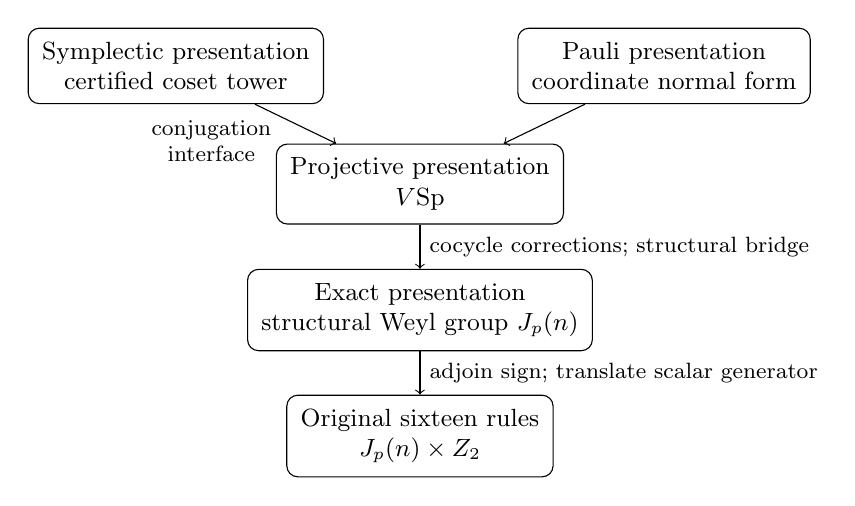
\begin{tikzpicture}[
 box/.style={draw,rounded corners,align=center,font=\small,inner sep=5pt},
 lab/.style={font=\footnotesize,align=center}]
\node[box] (sp) at (0,0) {Symplectic presentation\\certified coset tower};
\node[box] (pauli) at (6.2,0) {Pauli presentation\\coordinate normal form};
\node[box] (proj) at (3.1,-1.5) {Projective presentation\\$V\rtimes\mathrm{Sp}$};
\node[box] (exact) at (3.1,-3.1) {Exact presentation\\structural Weyl group $J_p(n)$};
\node[box] (signed) at (3.1,-4.7) {Original sixteen rules\\$J_p(n)\times\mathbb Z_2$};
\draw[->] (sp) -- (proj);
\node[lab] at (0.45,-0.95) {conjugation\\interface};
\draw[->] (pauli) -- (proj);
\draw[->] (proj) -- node[lab,right]{cocycle corrections; structural bridge} (exact);
\draw[->] (exact) -- node[lab,right]{adjoin sign; translate scalar generator} (signed);
\end{tikzpicture}
\caption{The semantic dependencies. Presentation translations change
the syntax at each layer without repeating the symplectic normalizer.
All arrows are checked; the correspondence to complex matrices is
outside the diagram.}
\label{fig:route}
\Description{The symplectic and Pauli presentations combine into the
projective group. A checked scalar extension and structural bridge give
the Weyl group. Adjoining a sign and translating generators recovers
the original circuit rules.}
\end{figure}
